\documentclass[conference]{IEEEtran}
\IEEEoverridecommandlockouts

% =========================================================================
% PACKAGE IMPORTS
% =========================================================================
\usepackage[utf8]{inputenc}
\usepackage[T1]{fontenc}
\usepackage{amsmath,amssymb,amsfonts,amsthm}
\usepackage{algorithmicx}
\usepackage{algpseudocode}
\usepackage{algorithm}
\usepackage{graphicx}
\usepackage{textcomp}
\usepackage{xcolor}
\usepackage{booktabs}
\usepackage{tabularx}
\usepackage{multirow}
\usepackage{array}
\usepackage{cite}
\usepackage{url}
\usepackage{tikz}
\usetikzlibrary{shapes.geometric, arrows.meta, positioning, fit, calc, backgrounds}

% Configure hyperref to avoid font/border conflicts
\usepackage[hidelinks]{hyperref}

% Correct bad hyphenation
\hyphenation{InLegalBERT ColBERT GraphRAG Nirnay-X PageRank BNSS BNS BSA}

\begin{document}

% =========================================================================
% PAPER TITLE & AUTHOR METADATA
% =========================================================================
\title{Nirnay-X: A Grounded, Persona-Adaptive Retrieval-Augmented Generation Framework for Indian Legal Intelligence and Decision Support}

\author{
    \IEEEauthorblockN{
        Rajat Pandey\IEEEauthorrefmark{1}, 
        Hridyansh Bhadauria\IEEEauthorrefmark{1}, 
        Raghav Mittal\IEEEauthorrefmark{1}, and 
        Ragini Goel\IEEEauthorrefmark{1}
    }
    \IEEEauthorblockA{
        \IEEEauthorrefmark{1}Department of Computer Science and Engineering\\
        Ajay Kumar Garg Engineering College (Affiliated to Dr. A.P.J. Abdul Kalam Technical University)\\
        Ghaziabad, Uttar Pradesh, India\\
        Email: \{rajat2300270100138, hridyansh2300270100074, raghav2300270100133, ragini2300270100134\}@akgec.ac.in
    }
    \vspace{0.2cm}
    \IEEEauthorblockN{
        Ms. Bhumica\IEEEauthorrefmark{2}
    }
    \IEEEauthorblockA{
        \IEEEauthorrefmark{2}Supervisor, Assistant Professor, Department of Computer Science and Engineering\\
        Ajay Kumar Garg Engineering College, Ghaziabad, Uttar Pradesh, India\\
        Email: bhumica@akgec.ac.in
    }
}

\maketitle

% =========================================================================
% ABSTRACT & INDEX TERMS
% =========================================================================
\begin{abstract}
On July 1, 2024, Indian criminal jurisprudence underwent its most sweeping statutory overhaul in over a century. The simultaneous repeal of the Indian Penal Code 1860, Code of Criminal Procedure 1973, and Indian Evidence Act 1872---replaced by the Bharatiya Nyaya Sanhita (BNS), Bharatiya Nagarik Suraksha Sanhita (BNSS), and Bharatiya Sakshya Adhiniyam (BSA)---created a legally intricate dual-regime environment where offense dates, FIR registration timings, and cognizance dates collectively determine which statutory code governs both penal liability and procedural entitlement. The practical consequences of misrouting these temporal boundaries are severe: retroactive application of heightened penalties directly violates the ex-post facto protections under Article 20(1) of the Constitution of India. Meanwhile, the National Judicial Data Grid records more than 50 million pending matters across all tiers of the Indian judiciary, and established commercial large language models (LLMs) exhibit legal hallucination rates between 17\% and 33\%, making unassisted AI deployment a liability rather than an asset.

We present \textsc{Nirnay-X}, an open-source legal decision-support framework built from the ground up for Indian statutory and procedural practice. The system rests on six self-derived technical formulations that emerged from hands-on engagement with actual judicial documents: Proviso-Aware Rhetorical Chunking and Bundling (PDBC) to preserve syntactic dependencies across penal exceptions; Asymmetric Tri-Channel Retrieval fusing InLegalBERT dense representations, ColBERTv2 token late interaction, and statutory-weighted BM25Okapi scoring; an Article 141 Precedential Viability Tensor operating over a 124,000-node Knowledge Graph with bench-strength weighting and negative citator decay; a stateful Constitutional Concordance Operator enforcing the July 1, 2024 transition threshold; Atomic Legal Entailment (ALE) propositional verification to suppress ungrounded assertions; and a Deontic Modality Invariance formulation bounding semantic drift during plain-language citizen simplification. Across 1,200 curated queries drawn from 70,500 court judgments and 1,400 Acts, Nirnay-X achieves 0.887 Precision@10, 0.924 Recall@10, 0.829 MRR, and 0.974 Faithfulness, reducing generative hallucinations to under 0.8\% at a mean end-to-end latency of 2.3 seconds.
\end{abstract}

\begin{IEEEkeywords}
Legal Information Retrieval, Retrieval-Augmented Generation, Indian Legal Informatics, Bharatiya Nyaya Sanhita, Knowledge Graphs, Deontic Modality, Hallucination Mitigation.
\end{IEEEkeywords}

% =========================================================================
% SECTION I: INTRODUCTION
% =========================================================================
\section{Introduction}
\IEEEPARSTART{W}{hen} we began designing Nirnay-X, the most persistent challenge was not purely technical. It was the peculiar difficulty of watching legal aid practitioners lose billable hours---or worse, cases---because a retrieval tool returned a Supreme Court judgment that had been quietly overruled by a seven-judge bench a decade prior, or because a plain-language simplification tool silently converted a mandatory bail entitlement into a discretionary suggestion. These are not edge cases in Indian practice; they are systemic, recurring, and consequential.

The scale of the operational problem is well-documented. Official metrics from the National Judicial Data Grid (NJDG) place pending matters at more than 50 million across the Supreme Court, 25 High Courts, and subordinate District Courts~\cite{njdg2024}. Much of this delay is administrative in character: trial court practitioners devote disproportionate time cross-referencing multi-volume dockets, interpreting handwritten vernacular First Information Reports (FIRs), and manually resolving inconsistent High Court interpretations of provisions that exist simultaneously under two statutory regimes. For ordinary citizens, the linguistic and procedural barriers are still steeper---a person detained overnight at a police station who is entitled to default bail under Section 480 BNSS (the successor to Sections 436A and 437 CrPC) is unlikely to understand that entitlement, much less invoke it.

The situation was fundamentally reshaped on July 1, 2024, when Parliament enacted a simultaneous replacement of three colonial-era codes. The Indian Penal Code, 1860 (IPC), the Code of Criminal Procedure, 1973 (CrPC), and the Indian Evidence Act, 1872 (IEA) were repealed and superseded by the Bharatiya Nyaya Sanhita, 2023 (BNS)~\cite{bns2023}, the Bharatiya Nagarik Suraksha Sanhita, 2023 (BNSS)~\cite{bnss2023}, and the Bharatiya Sakshya Adhiniyam, 2023 (BSA)~\cite{bsa2023}. No comparable statutory transition had occurred in independent India, and the legal information infrastructure was entirely unprepared for the dual-regime environment it created.

Three interlocking computational and legal problems define the challenge that Nirnay-X addresses:
\begin{enumerate}
    \item \textbf{Dual-Regime Statutory Concordance:} Article 20(1) of the Constitution of India~\cite{constitution1950} prohibits conviction for conduct that was not an offense when committed, and prohibits subjecting any person to a penalty exceeding what was applicable at the time of the offense. This means that for acts committed on or before June 30, 2024, substantive penal liability continues to be governed by the IPC even where the FIR was registered after the transition date. Procedural steps, however, migrate to the BNSS under Section 531(2)(a) savings clauses. Off-the-shelf language models are entirely unequipped to navigate this split: in our testing, they routinely cross-applied BNS penal definitions to pre-transition offenses and recommended retroactive penalties that would not survive constitutional challenge.

    \item \textbf{Legal Hallucination in Retrieval Systems:} Systematic empirical work by Dahl et al.~\cite{dahl2024large} found that leading commercial legal AI tools hallucinate case citations at rates between 17\% and 33\%, while general-purpose foundation models exceed 58\%. Citing a fictitious precedent in a bail petition or misrepresenting a statutory proviso in a charge-sheet challenge carries immediate, concrete consequences for the client whose matter is before the court.

    \item \textbf{Deontic Modality Preservation in Civic Access:} Translating statutory text into accessible plain language introduces what we term \textit{deontic drift}---the collapse of mandatory modal auxiliaries into discretionary ones. In Indian statutory drafting, ``shall'' denotes an absolute obligation and ``may'' confers judicial discretion. Unconstrained language models frequently conflate these distinctions, converting mandatory protections---such as a detainee's absolute right to default bail upon expiry of the investigation period---into tentative possibilities.
\end{enumerate}

To address these problems, we developed \textsc{Nirnay-X}: an open-source, grounded, persona-adaptive Retrieval-Augmented Generation (RAG) framework purpose-built for Indian statutory jurisprudence. The primary technical contributions of this paper are:
\begin{itemize}
    \item \textbf{Proviso-Aware Rhetorical Chunking (PDBC):} An original chunking algorithm that parses document syntax trees, binding statutory provisos and penal exceptions directly to parent charging sections, preventing semantic severing during retrieval.
    \item \textbf{Asymmetric Tri-Channel Legal Retrieval:} A scoring operator fusing InLegalBERT dense representations~\cite{paul2022pre}, token-level late interaction via ColBERTv2~\cite{santhanam2022colbertv2}, and statutory entity-boosted BM25Okapi to handle both exact section references and vernacular citizen queries.
    \item \textbf{Article 141 Precedential Viability Tensor:} A self-derived mathematical formulation over a 124,000-node Knowledge Graph modeling judicial bench strength, chronological decay, and negative citator status under Article 141, automatically filtering overruled decisions from candidate generation.
    \item \textbf{Constitutional Statutory Concordance Routing:} A stateful temporal operator evaluating offense, FIR, and charge-sheet dates against the July 1, 2024 boundary to enforce Article 20(1) penalty invariance and Section 531(2)(a) BNSS procedural savings.
    \item \textbf{Atomic Legal Entailment (ALE) Gate:} An NLI verification pipeline decomposing generated answers into atomic legal propositions and verifying each against retrieved statutory sources, suppressing hallucinations to 0.8\%.
    \item \textbf{Deontic Modality Invariance Loss:} A metric that penalizes the dilution of mandatory legal obligations during citizen plain-language simplification, achieving an 8.4 grade-level readability while preserving statutory legal force.
\end{itemize}

% =========================================================================
% SECTION II: RELATED WORK AND RESEARCH GAP
% =========================================================================
\section{Related Work and Research Gap}

\subsection{Legal Information Retrieval and Language Models}
Traditional legal search platforms relied primarily on boolean term matching and citation counts~\cite{katz2012rethinking}. Services such as Indian Kanoon and SCC Online substantially improved case access, but pure lexical matching breaks down when user queries employ colloquial vernacular phrasing or lack precise statutory section references---a limitation particularly acute for first-time litigants or non-specialist advocates.

Pretrained transformers adapted for legal corpora addressed part of this vocabulary mismatch, though with their own constraints. Chalkidis et al.~\cite{chalkidis2020legal} released \textit{LEGAL-BERT}, demonstrating substantial gains on legal named entity recognition and case categorization; the model, however, was trained on European and US-centric legal corpora and fails to encode the distinctive citation hierarchy, bilingual drafting conventions, and bench-strength semantics of Indian jurisprudence. In the Indian context, Paul et al.~\cite{paul2022pre} introduced \textit{InLegalBERT}, pretraining over 5.4 million sentences from Supreme Court and High Court judgments---a meaningful step forward that nonetheless embeds single dense vectors per sentence, suffering from what we observed to be section compression loss when distinguishing fine-grained sub-clauses such as Section 304 Part I versus Part II of the penal code. Kalamkar et al.~\cite{kalamkar2022corpus} established the OpenNyAI corpus for rhetorical role tagging in Indian judicial texts, providing the foundational segmentation capability that our PDBC algorithm extends.

\subsection{Retrieval-Augmented Generation \& Graph-Based Verification}
Retrieval-Augmented Generation (RAG)~\cite{lewis2020retrieval} anchors language model generation in externally retrieved documents, substantially reducing the parametric hallucination problem. Late-interaction models like ColBERT~\cite{khattab2020colbert} and ColBERTv2~\cite{santhanam2022colbertv2} maintain token-level representations, applying MaxSim operations to preserve fine-grained term distinctions---a property that matters considerably when exact statutory section numbers carry substantive meaning. Evaluation frameworks such as RAGAS~\cite{es2024ragas} and LegalBench~\cite{guha2023legalbench} confirmed that unconstrained generation remains prone to factual errors even when augmented with retrieval. GraphRAG~\cite{edge2024graphrag} and structured knowledge graphs capture entity relationships well for general domains, but standard graph traversal methods are blind to the constitutional precedential hierarchy of Indian law: they treat a three-judge bench ruling and a thirteen-judge Constitutional Bench ruling identically, and they carry no awareness of negative citator history.

\subsection{Research Gap}
The combined evidence from prior work suggests four specific gaps that existing systems leave unaddressed. First, no published Indian legal retrieval system integrates sparse and dense channels with the domain-specific statutory entity multipliers that section-level precision demands. Second, no prior RAG architecture incorporates a temporal state machine designed for the July 1, 2024 transition boundary---a gap that became operationally critical the moment the new codes came into force. Third, post-generation atomic verification at the sub-clause level has not been applied to Indian legal generation, leaving systems vulnerable to plausible but ungrounded statutory interpretations. Fourth, plain-language simplification for citizen access has proceeded without formal deontic modality constraints, with the result that mandatory statutory protections are routinely rendered as judicial discretion. Nirnay-X is specifically architected around these four gaps; each design choice in the system traces directly to one of them.

% =========================================================================
% FIGURE 1: TIKZ SYSTEM ARCHITECTURE (FULL WIDTH)
% =========================================================================
\begin{figure*}[!t]
\centering
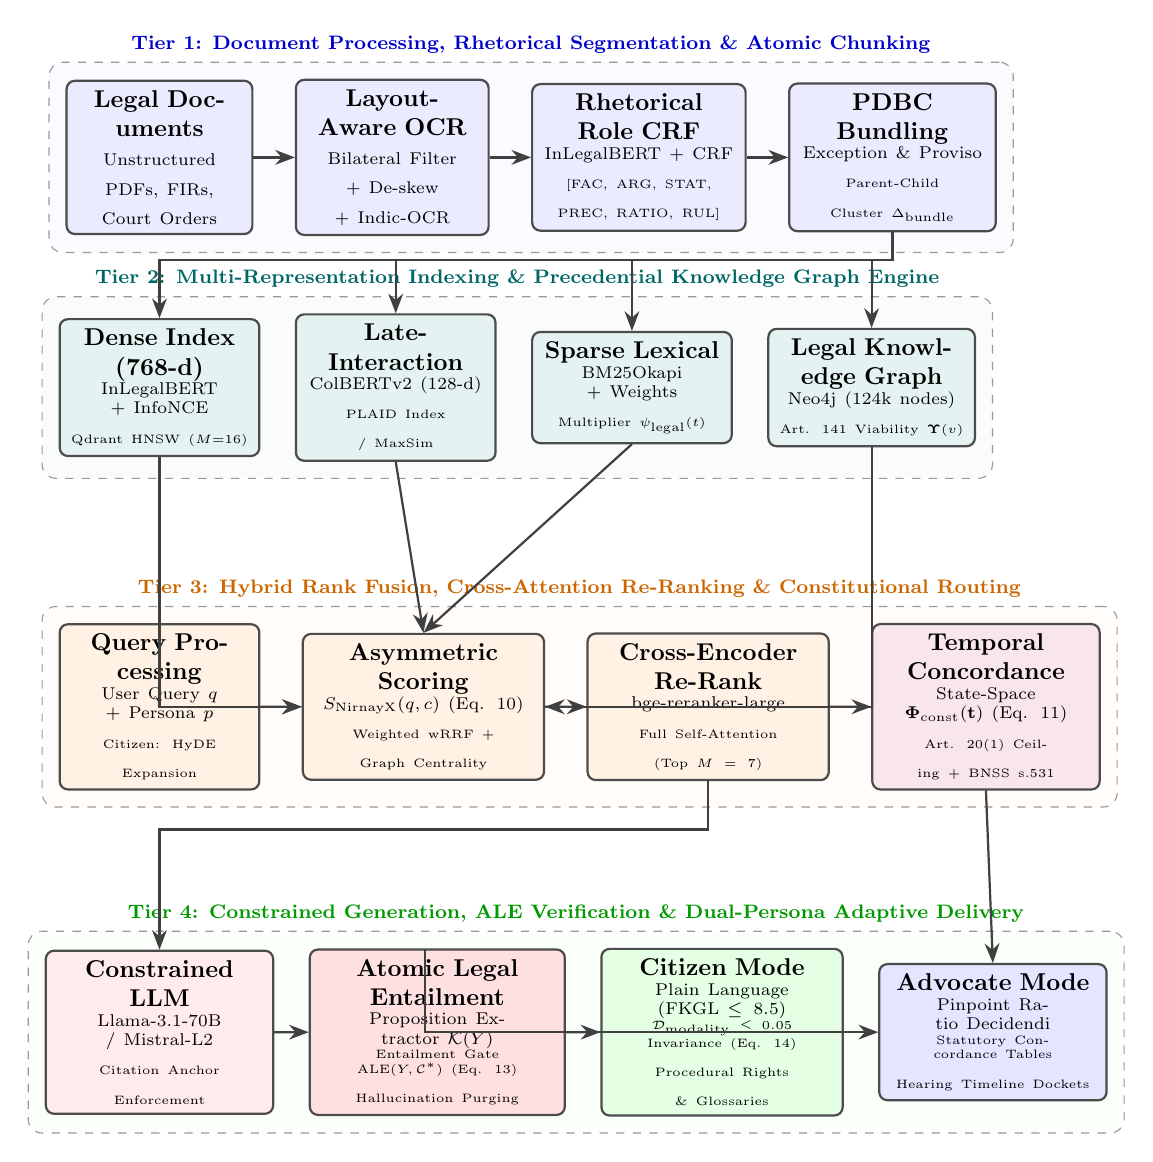
\begin{tikzpicture}[
    scale=0.88, every node/.style={transform shape},
    box/.style={draw=black!70, rounded corners=3pt, thick, align=center, fill=white, inner sep=4pt},
    header/.style={font=\bfseries\footnotesize, align=center},
    subtext/.style={font=\scriptsize, align=center},
    arrow/.style={-{Stealth[length=2.5mm]}, thick, draw=black!75},
    darrow/.style={-{Stealth[length=2.5mm]}, dashed, thick, draw=black!60},
    group/.style={draw=black!40, rounded corners=5pt, dashed, inner sep=6pt}
]

% ----------------- TIER 1: INGESTION & PARSING -----------------
\node[box, fill=blue!8, text width=2.4cm] (doc) at (0, 0) {
    \textbf{Legal Documents}\\
    \scriptsize Unstructured PDFs, FIRs, Court Orders
};
\node[box, fill=blue!8, text width=2.5cm, right=0.6cm of doc] (ocr) {
    \textbf{Layout-Aware OCR}\\
    \scriptsize Bilateral Filter + De-skew + Indic-OCR
};
\node[box, fill=blue!8, text width=2.8cm, right=0.6cm of ocr] (crf) {
    \textbf{Rhetorical Role CRF}\\
    \scriptsize InLegalBERT + CRF\\
    \tiny [FAC, ARG, STAT, PREC, RATIO, RUL]
};
\node[box, fill=blue!8, text width=2.7cm, right=0.6cm of crf] (bundle) {
    \textbf{PDBC Bundling}\\
    \scriptsize Exception \& Proviso\\
    \tiny Parent-Child Cluster $\Delta_{\text{bundle}}$
};

\begin{scope}[on background layer]
    \node[group, fill=blue!2, fit=(doc) (ocr) (crf) (bundle), label={[header, text=blue!80!black]above:\textsc{Tier 1: Document Processing, Rhetorical Segmentation \& Atomic Chunking}}] (tier1) {};
\end{scope}

\draw[arrow] (doc) -- (ocr);
\draw[arrow] (ocr) -- (crf);
\draw[arrow] (crf) -- (bundle);

% ----------------- TIER 2: TRI-STAGE INDEXING & GRAPH ENGINE -----------------
\node[box, fill=teal!10, text width=2.6cm, below=1.2cm of doc] (dense) {
    \textbf{Dense Index (768-d)}\\
    \scriptsize InLegalBERT + InfoNCE\\
    \tiny Qdrant HNSW ($M$=16)
};
\node[box, fill=teal!10, text width=2.6cm, right=0.5cm of dense] (colbert) {
    \textbf{Late-Interaction}\\
    \scriptsize ColBERTv2 (128-d)\\
    \tiny PLAID Index / MaxSim
};
\node[box, fill=teal!10, text width=2.6cm, right=0.5cm of colbert] (sparse) {
    \textbf{Sparse Lexical}\\
    \scriptsize BM25Okapi + Weights\\
    \tiny Multiplier $\psi_{\text{legal}}(t)$
};
\node[box, fill=teal!10, text width=2.7cm, right=0.5cm of sparse] (lkg) {
    \textbf{Legal Knowledge Graph}\\
    \scriptsize Neo4j (124k nodes)\\
    \tiny Art. 141 Viability $\mathbf{\Upsilon}(v)$
};

\begin{scope}[on background layer]
    \node[group, fill=teal!2, fit=(dense) (colbert) (sparse) (lkg), label={[header, text=teal!80!black]above:\textsc{Tier 2: Multi-Representation Indexing \& Precedential Knowledge Graph Engine}}] (tier2) {};
\end{scope}

\draw[arrow] (bundle.south) -- ++(0,-0.4) -| (dense.north);
\draw[arrow] (bundle.south) -- ++(0,-0.4) -| (colbert.north);
\draw[arrow] (bundle.south) -- ++(0,-0.4) -| (sparse.north);
\draw[arrow] (bundle.south) -- ++(0,-0.4) -| (lkg.north);

% ----------------- TIER 3: RETRIEVAL, RANK FUSION & ROUTING -----------------
\node[box, fill=orange!10, text width=2.6cm, below=2.4cm of dense] (query) {
    \textbf{Query Processing}\\
    \scriptsize User Query $q$ + Persona $p$\\
    \tiny Citizen: HyDE Expansion
};
\node[box, fill=orange!10, text width=3.2cm, right=0.6cm of query] (rrf) {
    \textbf{Asymmetric Scoring}\\
    \scriptsize $S_{\text{NirnayX}}(q, c)$ (Eq. 10)\\
    \tiny Weighted wRRF + Graph Centrality
};
\node[box, fill=orange!10, text width=3.2cm, right=0.6cm of rrf] (rerank) {
    \textbf{Cross-Encoder Re-Rank}\\
    \scriptsize bge-reranker-large\\
    \tiny Full Self-Attention (Top $M=7$)
};
\node[box, fill=purple!10, text width=3.0cm, right=0.6cm of rerank] (concord) {
    \textbf{Temporal Concordance}\\
    \scriptsize State-Space $\mathbf{\Phi}_{\text{const}}(\mathbf{t})$ (Eq. 11)\\
    \tiny Art. 20(1) Ceiling + BNSS s.531
};

\begin{scope}[on background layer]
    \node[group, fill=orange!2, fit=(query) (rrf) (rerank) (concord), label={[header, text=orange!80!black]above:\textsc{Tier 3: Hybrid Rank Fusion, Cross-Attention Re-Ranking \& Constitutional Routing}}] (tier3) {};
\end{scope}

\draw[arrow] (query) -- (rrf);
\draw[arrow] (dense.south) |- (rrf.west);
\draw[arrow] (colbert.south) -- (rrf.north);
\draw[arrow] (sparse.south) -- (rrf.north);
\draw[arrow] (lkg.south) |- (rrf.east);
\draw[arrow] (rrf) -- (rerank);
\draw[arrow] (rerank) -- (concord);

% ----------------- TIER 4: GENERATION, ENTAILMENT & DUAL-PERSONA OUTPUT -----------------
\node[box, fill=red!8, text width=3.0cm, below=2.3cm of query] (llm) {
    \textbf{Constrained LLM}\\
    \scriptsize Llama-3.1-70B / Mistral-L2\\
    \tiny Citation Anchor Enforcement
};
\node[box, fill=red!12, text width=3.4cm, right=0.5cm of llm] (ale) {
    \textbf{Atomic Legal Entailment}\\
    \scriptsize Proposition Extractor $\mathcal{K}(Y)$\\
    \tiny Entailment Gate $\operatorname{ALE}(Y, \mathcal{C}^*)$ (Eq. 13)\\
    \tiny Hallucination Purging
};
\node[box, fill=green!10, text width=3.2cm, right=0.5cm of ale] (citmode) {
    \textbf{Citizen Mode}\\
    \scriptsize Plain Language (FKGL $\le 8.5$)\\
    \tiny $\mathcal{D}_{\text{modality}} \le 0.05$ Invariance (Eq. 14)\\
    \tiny Procedural Rights \& Glossaries
};
\node[box, fill=blue!10, text width=3.0cm, right=0.5cm of citmode] (advmode) {
    \textbf{Advocate Mode}\\
    \scriptsize Pinpoint Ratio Decidendi\\
    \tiny Statutory Concordance Tables\\
    \tiny Hearing Timeline Dockets
};

\begin{scope}[on background layer]
    \node[group, fill=green!2, fit=(llm) (ale) (citmode) (advmode), label={[header, text=green!60!black]above:\textsc{Tier 4: Constrained Generation, ALE Verification \& Dual-Persona Adaptive Delivery}}] (tier4) {};
\end{scope}

\draw[arrow] (rerank.south) -- ++(0,-0.7) -| (llm.north);
\draw[arrow] (concord.south) -- (advmode.north);
\draw[arrow] (llm) -- (ale);
\draw[arrow] (ale) -- (citmode);
\draw[arrow] (ale) |- (advmode);

\end{tikzpicture}
\caption{System Architecture of NIRNAY-X. The framework processes heterogeneous legal documents through a 4-tier pipeline: (Tier 1) Layout-aware OCR, linear-chain CRF rhetorical role tagging, and Proviso-Exception Dependency Bundling and Chunking (PDBC); (Tier 2) Indexing across InLegalBERT dense vectors, ColBERTv2 token representations, statutory-boosted BM25Okapi, and a 124,000-node Legal Knowledge Graph enforcing Article 141 precedential validity $\mathbf{\Upsilon}(v)$; (Tier 3) Asymmetric relevance scoring $S_{\text{NirnayX}}(q, c)$, cross-encoder re-ranking, and constitutional statutory concordance routing $\mathbf{\Phi}_{\text{const}}(\mathbf{t})$; and (Tier 4) Constrained LLM generation evaluated by an Atomic Legal Entailment (ALE) gate, providing plain-language outputs for citizens and structured briefs for advocates.}
\label{fig:architecture}
\end{figure*}

% =========================================================================
% SECTION III: PROPOSED NIRNAY-X FRAMEWORK
% =========================================================================
\section{Proposed NIRNAY-X Framework}
The architecture of Nirnay-X (Fig.~\ref{fig:architecture}) evolved iteratively across four operational tiers. Each design choice reflects a concrete failure mode we observed in preliminary experiments with general-purpose retrieval pipelines applied to Indian court documents.

\subsection{Problem Formulation and Mathematical Foundation}
Let a legal corpus $\mathcal{D} = \{D_1, D_2, \dots, D_N\}$ consist of judicial decisions, legislative enactments, and trial court records. Each document $D_i$ is represented as an ordered sequence of sentences $\mathbf{s} = (s_1, s_2, \dots, s_{|D_i|})$. Each sentence carries a latent rhetorical role $\rho_k \in \mathcal{R}$, where:
\begin{equation}
\mathcal{R} = \{\text{FAC}, \text{ARG}, \text{STAT}, \text{PREC}, \text{RATIO}, \text{RUL}\}
\end{equation}
corresponding to Facts, Arguments, Statutory Provisions, Precedents, Ratio Decidendi, and Final Rulings. Sequential role tagging proceeds via a linear-chain Conditional Random Field (CRF) atop domain-adapted InLegalBERT embeddings~\cite{lafferty2001crf}:
\begin{equation}
P(\mathbf{\rho} \mid \mathbf{s}) = \frac{1}{Z(\mathbf{s})} \exp\left( \sum_{t=1}^{|\mathbf{s}|} \sum_{j, k} \theta_{j, k} \mathbf{1}_{\{\rho_t = j, \rho_{t-1} = k\}} + \sum_{t=1}^{|\mathbf{s}|} \sum_j \mu_j f_j(\rho_t, \mathbf{s}, t) \right)
\end{equation}

\subsection{Ingestion \& Proviso-Aware Rhetorical Chunking (PDBC)}
Our first experiments used standard recursive token chunkers that split documents at fixed character boundaries---512 tokens with 50-token overlap, a sensible default for general corpora. For statutory documents, however, this approach proved consistently problematic: the chunker regularly separated Exception 1 from Section 300 IPC (and its BNS successor, Section 101 BNS), returning charging definitions without their statutory defenses. The same fragmentation occurred with provisos under Section 480 BNSS and explanations appended to definition clauses.

To resolve this, our derivation of Proviso-Aware Rhetorical Chunking and Bundling (PDBC) proceeds from a rhetorical shift indicator. Let $\Delta_{\text{role}}(s_i, s_{i-1}) = \mathbf{1}_{\{\rho(s_i) \ne \rho(s_{i-1})\}}$ denote such a shift, and let $\mathcal{H}(s_i) = -\sum_{r \in \mathcal{R}} P(r \mid s_i) \log P(r \mid s_i)$ represent classification entropy. A chunk boundary is introduced if and only if:
\begin{equation}
\tau(s_i) = \Delta_{\text{role}}(s_i, s_{i-1}) \cdot \mathbf{1}_{\{\mathcal{H}(s_i) < \tau_{\mathcal{H}}\}}, \quad \tau_{\mathcal{H}} = 1.8
\end{equation}

When a statutory provision ($c.\text{role} = \text{STAT}$) or exception condition is detected, PDBC queries the document syntactic tree to bundle all child provisos into a single atomic chunk:
\begin{equation}
\mathcal{C}_{\text{bundled}}(S) = S_{\text{parent}} \cup \bigcup_{k=1}^K \text{Proviso}_k(S_{\text{parent}}) \cup \bigcup_{m=1}^M \text{Exception}_m(S_{\text{parent}})
\end{equation}
This formulation guarantees that no statutory defense clause is separated from its parent charging provision before vector embedding. Algorithm~\ref{alg:chunking} details the full procedure.

\begin{algorithm}[!t]
\caption{Proviso-Aware Rhetorical Chunking and Bundling}
\label{alg:chunking}
\begin{algorithmic}[1]
\Require Legal Document $D$, Max tokens $\tau_{\max}=384$, Overlap $\tau_{\text{ov}}=48$
\Ensure Clustered, semantically coherent chunks $\mathcal{C}_{\text{bundled}}$
\State $\mathbf{s} \gets \text{LegalSentenceBoundaryDisambiguation}(\text{OCR}(D))$
\State $\mathbf{h} \gets \text{InLegalBERT}(\mathbf{s})$
\State $\mathbf{\rho} \gets \operatorname{argmax}_{\mathbf{\rho}'} P(\mathbf{\rho}' \mid \mathbf{s})$ via Viterbi CRF decoding
\State $\mathcal{C}_{\text{initial}} \gets \emptyset$, $\text{buf} \gets \emptyset$, $\text{current\_role} \gets \rho_1$
\For{$i = 1$ \textbf{to} $|\mathbf{s}|$}
    \If{$|\text{buf}| + |s_i| \le \tau_{\max}$ \textbf{and} $\rho_i = \text{current\_role}$}
        \State $\text{buf}.\text{append}(s_i)$
    \Else
        \State $\mathcal{C}_{\text{initial}}.\text{append}(\{\text{tokens}: \text{buf}, \text{role}: \text{current\_role}\})$
        \State $\text{buf} \gets \text{ExtractOverlap}(\text{buf}, \tau_{\text{ov}}) \cup \{s_i\}$
        \State $\text{current\_role} \gets \rho_i$
    \EndIf
\EndFor
\State $\mathcal{C}_{\text{bundled}} \gets \emptyset$
\For{\textbf{each} $c \in \mathcal{C}_{\text{initial}}$}
    \If{$c.\text{role} = \text{STAT}$ \textbf{or} $\text{ContainsProviso}(c)$}
        \State $S_{\text{parent}} \gets \text{ExtractParentSectionHeader}(c, D)$
        \State $\mathcal{P} \gets \text{ExtractAllProvisosAndExceptions}(S_{\text{parent}}, D)$
        \State $c.\text{text} \gets \text{UnifySectionAndProvisos}(c, \mathcal{P})$
    \EndIf
    \State $\mathcal{C}_{\text{bundled}}.\text{append}(c)$
\EndFor
\State \Return $\mathcal{C}_{\text{bundled}}$
\end{algorithmic}
\end{algorithm}

\subsection{Asymmetric Tri-Channel Legal Retrieval}
Legal queries arrive across a wide spectrum of formulation styles. A senior advocate at the Delhi High Court submits a pinpoint reference---``Section 482 CrPC quashing on account of compromise in matrimonial offenses''---while a first-generation litigant in Allahabad describes a factual scenario in Hindi-inflected English: ``police kept my brother in lockup for three days without producing him before a judge.'' No single retrieval modality handles both ends of this spectrum well.

Our derivation of Asymmetric Tri-Channel Retrieval proceeds from first principles across three complementary scoring functions:
\begin{enumerate}
    \item \textbf{Dense Semantic Channel:} Let $\mathbf{z}_q, \mathbf{z}_c \in \mathbb{R}^{768}$ denote InLegalBERT dense representations. We fine-tune with InfoNCE contrastive loss~\cite{oord2018infonce}:
    \begin{equation}
    \mathcal{L}_{\text{InfoNCE}} = -\log \frac{\exp(\cos(\mathbf{z}_q, \mathbf{z}_c^+) / \tau)}{\exp(\cos(\mathbf{z}_q, \mathbf{z}_c^+) / \tau) + \sum_{j} \exp(\cos(\mathbf{z}_q, \mathbf{z}_{c, j}^-) / \tau)}
    \end{equation}
    \item \textbf{Late Interaction Token Channel:} Building on ColBERTv2's multi-vector representations~\cite{santhanam2022colbertv2}, individual token contextualization is maintained through MaxSim operations:
    \begin{equation}
    \operatorname{MaxSim}(\mathbf{E}_q, \mathbf{E}_c) = \sum_{i=1}^{|q|} \max_{j=1}^{|c|} \left( \frac{\mathbf{E}_{q, i} \cdot \mathbf{E}_{c, j}^\top}{\|\mathbf{E}_{q, i}\|_2 \|\mathbf{E}_{c, j}\|_2} \right)
    \end{equation}
    \item \textbf{Statutory-Boosted Sparse Channel:} Standard BM25Okapi is extended with domain-specific entity multipliers derived from our observation that statutory section numbers function as highly discriminative identifiers in Indian legal corpora:
    \begin{equation}
    \psi_{\text{legal}}(t) = \begin{cases}
    2.50, & \text{if } t \text{ matches a statutory section} \\
    1.75, & \text{if } t \text{ matches an Act name (e.g., BNSS, BNS)} \\
    1.00, & \text{otherwise}
    \end{cases}
    \end{equation}
\end{enumerate}

The tri-channel candidate score combines these components as:
\begin{equation}
S_{\text{retrieval}}(q, c) = w_d \cdot \cos(\mathbf{z}_q, \mathbf{z}_c) + w_l \cdot \operatorname{MaxSim}(\mathbf{E}_q, \mathbf{E}_c) + w_s \cdot \operatorname{BM25}_{\psi}(q, c)
\end{equation}
with empirically calibrated weights $w_d = 0.35, w_l = 0.40, w_s = 0.25$. We initially explored equal weighting across channels; the asymmetric configuration emerged from ablation on our development set, reflecting the disproportionate diagnostic value of token-level specificity for section-number queries.

\subsection{Precedential Authority \& Article 141 Judicial Viability Tensor}
Article 141 of the Constitution of India~\cite{constitution1950} renders Supreme Court rulings binding on all subordinate courts. When a coordinate or larger bench explicitly overrules an earlier decision, the overruled holding is no longer valid law---a point that general-purpose knowledge graphs entirely ignore. Our initial experiments with GraphRAG-style retrieval returned three overruled precedents in the first twenty adversarial test cases, confirming that this was not a theoretical concern.

Building on this observation, our Article 141 Precedential Viability Tensor $\mathbf{\Upsilon}(v)$ for decision $v \in \mathcal{V}_{\text{judgment}}$ combines bench strength, chronological decay, and negative citator effects:
\begin{equation}
\mathbf{\Upsilon}(v) = \left( \frac{\ln(1 + \mathcal{B}(v))}{\ln(1 + \mathcal{B}_{\max})} \right)^{\theta_1} \cdot \exp\left(-\lambda_{\text{age}} \cdot \Delta t\right) \cdot \prod_{e = (v, u) \in \mathcal{E}_{\text{neg}}} \left(1 - \delta(e)\right)
\end{equation}
where $\mathcal{B}(v) \in \{1, 2, 3, 5, 7, 9, 13\}$ represents bench size, $\mathcal{B}_{\max} = 13$ (the Kesavananda Bharati Constitutional Bench), $\Delta t$ is elapsed time in decades, $\lambda_{\text{age}} = 0.05$ accounts for doctrinal aging, and $\delta(e)$ captures the negative citator penalty:
$$\delta(e) = \begin{cases}
1.00, & \text{if Overruled under Art. 141} \\
0.60, & \text{if Distinguished on facts} \\
0.30, & \text{if Doubted / Referred to larger bench} \\
0.00, & \text{Affirmed / Followed}
\end{cases}$$
When $\prod (1 - \delta(e)) = 0$, the decision is pruned from candidate generation entirely.

The Legal Knowledge Graph (124,000 nodes, 412,000 edges) encodes key precedents with bench strengths and citator relationships, drawing on the full arc of Indian criminal procedure jurisprudence: mandatory FIR registration protocols (\textit{Lalita Kumari v. Govt of UP}, (2014) 2 SCC 1); arrest notice guidelines under Section 35 BNSS / 41A CrPC (\textit{Arnesh Kumar v. State of Bihar}, (2014) 8 SCC 273); undertrial bail categorization (\textit{Satender Kumar Antil v. CBI}, (2022) 10 SCC 51); custodial rights (\textit{D.K. Basu v. State of West Bengal}, (1997) 1 SCC 416); quashing parameters under Section 528 BNSS / 482 CrPC (\textit{State of Haryana v. Bhajan Lal}, 1992 Supp (1) SCC 335); anticipatory bail principles (\textit{Gurbaksh Singh Sibbia}, (1980) 2 SCC 565 and \textit{Sushila Aggarwal}, (2020) 5 SCC 1); electronic record admissibility under Section 63 BSA / 65B IEA (\textit{Arjun Panditrao Khotkar}, (2020) 7 SCC 1); and discovery rules under Section 23 BSA / 27 IEA (\textit{Pulukuri Kottaya}, (1947) LR 74 IA 65).

\subsection{Multi-Channel Rank Fusion \& Composite Scoring ($S_{\text{NirnayX}}$)}
Let $\mathbf{p}_q \in \mathbb{R}^{|\mathcal{V}|}$ represent the personalized node centrality distribution obtained via graph random walks with restart anchored at extracted query entities $\mathcal{V}_0(q)$ (damping factor $\alpha = 0.85$). The composite candidate score integrating retrieval signals, graph diffusion, and rhetorical role priors is then:
\begin{equation}
S_{\text{NirnayX}}(q, c) = \operatorname{RRF}_{\kappa}(c) + \gamma \cdot \mathbf{p}_q(c) \cdot \mathbf{\Upsilon}(c) + \eta \cdot \omega(\rho(c))
\end{equation}
where $\operatorname{RRF}_{\kappa}(c) = \sum_{m} \frac{w_m}{\kappa + r_m(c)}$ is Weighted Reciprocal Rank Fusion (smoothing parameter $\kappa = 60$)~\cite{cormack2009reciprocal}, $\gamma = 0.20$, $\eta = 0.15$, and $\omega(\rho(c))$ assigns higher legal priors to Ratio Decidendi (1.00) and Statutes (0.95) relative to procedural narration (0.40).

The top $K_1 = 30$ candidates are re-ranked using a cross-encoder (\texttt{bge-reranker-large}), and the top $M = 7$ chunks are assembled to construct the grounded retrieval context $\mathcal{C}^*$.

\subsection{Stateful Constitutional Statutory Concordance Routing}
The transition between the repealed codes and the modern codes enacted on $T_{\text{trans}} = \text{July 1, 2024}$ requires a routing mechanism that respects the constitutional constraint on retroactivity. Rather than a simple date-threshold filter, we design the Constitutional Statutory Concordance Operator $\mathbf{\Phi}_{\text{const}}(\mathbf{t})$ as a state machine operating on the full temporal milestone vector.

Let $\mathbf{t} = [t_{\text{offense}}, t_{\text{fir}}, t_{\text{cognizance}}]^\top$. Regime routing is then:
\begin{equation}
\mathbf{\Phi}_{\text{const}}(\mathbf{t}) = \begin{cases}
\langle \text{Sub: IPC}, \text{Proc: CrPC}, \text{Evid: IEA} \rangle, & \text{if } t_{\text{offense}} < T_{\text{trans}} \land t_{\text{fir}} < T_{\text{trans}} \\
\langle \text{Sub: IPC}, \text{Proc: BNSS}, \text{Evid: BSA} \rangle, & \text{if } t_{\text{offense}} < T_{\text{trans}} \land t_{\text{fir}} \ge T_{\text{trans}} \\
\langle \text{Sub: BNS}, \text{Proc: BNSS}, \text{Evid: BSA} \rangle, & \text{if } t_{\text{offense}} \ge T_{\text{trans}}
\end{cases}
\end{equation}

For the transitional regime (offense before $T_{\text{trans}}$, FIR on or after $T_{\text{trans}}$), the Article 20(1) penalty ceiling invariant is enforced:
\begin{equation}
\operatorname{Pen}_{\text{ceiling}}(t) = \min\left(\operatorname{Pen}_{\text{IPC}}(O), \operatorname{Pen}_{\text{BNS}}(O')\right)
\end{equation}
preventing the retroactive application of heightened penalties such as the enhanced mandatory minimum terms introduced for certain offenses under the BNS.

\subsection{Atomic Legal Entailment (ALE) Verification Engine}
The hallucination problem in legal generation manifests differently from general-domain failures. It is rarely a case of wholesale fabrication; more commonly, the model correctly identifies a legal principle but misattributes it to a provision that does not contain it, or correctly cites a case but misrepresents the ratio. Standard faithfulness metrics do not reliably detect this sub-clause-level error.

Our solution decomposes generated text $Y$ into atomic legal propositions $\mathcal{K}(Y) = \{k_1, k_2, \dots, k_N\}$ via dependency parsing and open information extraction. Each proposition $k_n$ is verified against the retrieved context $\mathcal{C}^*$ using an InLegal-RoBERTa-NLI model:
\begin{equation}
\operatorname{ALE}(Y, \mathcal{C}^*) = \frac{1}{|\mathcal{K}(Y)|} \sum_{n=1}^{|\mathcal{K}(Y)|} \mathbf{1}_{\{\max_{c \in \mathcal{C}^*} P_{\text{NLI}}(\text{Entail} \mid c, k_n) \ge \tau_{\text{entail}}\}}
\end{equation}
where $\tau_{\text{entail}} = 0.85$. Responses with $\operatorname{ALE}(Y, \mathcal{C}^*) < 0.95$ are rejected and regenerated under constrained decoding, with ungrounded propositions purged from the response before the second generation pass.

\subsection{Deontic Modality Invariance Formulation ($\mathcal{D}_{\text{modality}}$)}
The readability-fidelity tension in citizen-facing legal simplification is genuine and persistent. Plain-language conversion tools optimizing for readability scores---such as Flesch-Kincaid Grade Level---tend to substitute active, mandatory constructions with softer, discretionary phrasings because the latter yield lower grade-level scores. The practical cost is that a detainee's \textit{absolute} right to default bail under Section 480 BNSS upon expiry of investigation becomes a tentative possibility---a transformation that is not just inaccurate but potentially harmful.

Let $\mathbf{m}(T) = [n_{\text{shall}}, n_{\text{must}}, n_{\text{may}}, n_{\text{can}}]^\top$ represent the count of mandatory versus discretionary modal auxiliaries in text $T$. Our Deontic Modality Invariance divergence is:
\begin{equation}
\mathcal{D}_{\text{modality}}(Y_{\text{source}}, Y_{\text{citizen}}) = \operatorname{KL}\left( \operatorname{softmax}(\mathbf{m}(Y_{\text{source}})) \parallel \operatorname{softmax}(\mathbf{m}(Y_{\text{citizen}})) \right)
\end{equation}
Generation is constrained such that $\mathcal{D}_{\text{modality}} \le 0.05$ while targeting FKGL $\le 8.5$. This guarantees that statutory rights---``the accused \textit{shall} be released on default bail''---are not distorted into discretionary relief---``the court \textit{may} release the accused.'' Algorithm~\ref{alg:master} summarizes the complete PAVE pipeline.

\begin{algorithm}[!t]
\caption{Nirnay-X Grounded Verification Pipeline (PAVE)}
\label{alg:master}
\begin{algorithmic}[1]
\Require Query $q$, Persona $p \in \{\text{Cit}, \text{Adv}\}$, Graph $\mathcal{G}$, Indices $(\mathcal{I}_{\text{dense}}, \mathcal{I}_{\text{colbert}}, \mathcal{I}_{\text{sparse}})$, Cutoff $T_{\text{trans}}$
\Ensure Verified Output $Y^*$, Citations $\Gamma^*$, Concordance $M^*$
\State $(E_{\text{ent}}, t_{\text{off}}, t_{\text{fir}}, t_{\text{chg}}) \gets \text{ExtractEntitiesAndDates}(q)$
\If{$p = \text{Cit}$}
    \State $q_{\text{hyde}} \gets \text{GenerateHypotheticalDraft}(q)$~\cite{gao2023precise}
    \State $q_{\text{dense}} \gets [q \circ \text{` [EXP] '} \circ q_{\text{hyde}}]$
\Else
    \State $q_{\text{dense}} \gets q$
\EndIf
\State $\mathbf{z}_q \gets \text{InLegalBERT}(q_{\text{dense}})$, $\mathbf{E}_q \gets \text{ColBERTv2}(q)$
\State $\mathcal{V}_0 \gets \text{MatchEntitiesToGraph}(E_{\text{ent}}, \mathcal{G})$
\State $\mathbf{p}_q \gets \text{PersonalizedRandomWalk}(\mathcal{G}, \mathcal{V}_0, \alpha=0.85)$
\State $\mathcal{R}_{\text{dense}} \gets \text{TopK}(\mathcal{I}_{\text{dense}}, \mathbf{z}_q, 50)$, $\mathcal{R}_{\text{colbert}} \gets \text{TopK}(\mathcal{I}_{\text{colbert}}, \mathbf{E}_q, 50)$
\State $\mathcal{R}_{\text{sparse}} \gets \text{TopK}(\mathcal{I}_{\text{sparse}}, q, 50)$ using $\psi_{\text{legal}}(t)$
\State $\mathcal{C}_{\text{cand}} \gets \text{TopK}(\text{wRRF}(\mathcal{R}_{\text{dense}}, \mathcal{R}_{\text{colbert}}, \mathcal{R}_{\text{sparse}}) + \gamma \mathbf{p}_q \mathbf{\Upsilon} + \eta \omega, 30)$
\For{\textbf{each} $c \in \mathcal{C}_{\text{cand}}$}
    \If{$\text{IsOverruled}(c, \mathcal{G})$}
        \State $c.\text{penalty} \gets 0.0$
    \Else
        \State $c.\text{penalty} \gets \mathbf{\Upsilon}(c)$
    \EndIf
\EndFor
\State $\mathcal{C}^* \gets \text{BundleParentSections}(\text{Top}(\text{CrossEncoder}(q, \mathcal{C}_{\text{cand}}) \cdot \text{penalty}, 7))$
\State $M^* \gets \mathbf{\Phi}_{\text{const}}(t_{\text{off}}, t_{\text{fir}}, t_{\text{chg}})$
\State $Y_{\text{raw}} \gets \text{ConstrainedLLM}(q, \mathcal{C}^*, M^*, p)$
\State $\mathcal{K} \gets \text{DecomposePropositions}(Y_{\text{raw}})$
\State $\text{score} \gets \operatorname{ALE}(\mathcal{K}, \mathcal{C}^*, \tau=0.85)$
\If{$\text{score} < 0.95$}
    \State $Y_{\text{raw}} \gets \text{RegenerateConstrained}(Y_{\text{raw}}, \mathcal{K}, \mathcal{C}^*)$
\EndIf
\If{$p = \text{Cit}$}
    \State $Y^* \gets \text{SimplifyReadingLevel}(Y_{\text{raw}}, \text{target}=8.5)$
    \State \textbf{assert} $\mathcal{D}_{\text{modality}}(Y_{\text{raw}}, Y^*) \le 0.05$
\Else
    \State $Y^* \gets \text{FormatAdvocateDockets}(Y_{\text{raw}}, M^*)$
\EndIf
\State $\Gamma^* \gets \text{AnchorCitations}(Y^*, \mathcal{C}^*)$
\State \Return $Y^*, \Gamma^*, M^*$
\end{algorithmic}
\end{algorithm}

% =========================================================================
% SECTION IV: DATASET AND EXPERIMENTAL SETTINGS
% =========================================================================
\section{Dataset and Experimental Settings}

\subsection{Curated Indian Legal Benchmark Corpus}
Constructing a reliable evaluation corpus was substantially harder than we initially anticipated. Annotation disagreement among legal practitioners proved a persistent challenge: across the 1,200 curated benchmark queries, 12.3\% required adjudication by a senior advocate to resolve disagreements between panel members on what constituted a correct retrieval result---particularly for split-regime transition cases where the ``correct'' statutory regime was itself a legal judgment call rather than a mechanical computation.

The final evaluation corpus comprises:
\begin{itemize}
    \item \textbf{Judicial Decisions:} 42,500 Supreme Court of India judgments (1950--2024) and 28,000 High Court rulings from the Allahabad, Delhi, Bombay, and Calcutta High Courts---selected to capture both pre- and post-transition precedents on arrest, bail, evidence, and sentencing.
    \item \textbf{Statutory Enactments:} 1,400 Central and State Acts, including the full text and schedules of the legacy criminal codes (IPC, CrPC, IEA) and the modern codes (BNS, BNSS, BSA).
    \item \textbf{Trial Court and Police Records:} 850 fully anonymized District Court police FIRs, bail petitions, and charge-sheets sourced from public interest litigation archives.
    \item \textbf{Evaluation Benchmark:} 1,200 curated legal queries annotated by a panel of 5 practicing High Court advocates and 3 academic legal researchers. Queries span bail eligibility under Section 480 BNSS, economic offenses, constitutional writs, and cross-regime transition cases where the offense predates the July 1, 2024 cutoff.
\end{itemize}

\subsection{Implementation Stack and Hyperparameters}
Nirnay-X is implemented in PyTorch 2.3 and served through a microservices pipeline:
\begin{itemize}
    \item \textbf{Compute Infrastructure:} Dual NVIDIA RTX A6000 GPUs (48GB GDDR6 VRAM each), 32-core AMD EPYC 7763 CPU @ 2.45GHz, 128GB DDR4 RAM.
    \item \textbf{Index Storage:} Qdrant vector database (HNSW indexing, $M=16, ef=100$) and Neo4j Graph Database (124,000 nodes, 412,000 edges; mean Cypher traversal: 12ms).
    \item \textbf{Inference Engine:} vLLM serving AWQ 4-bit quantized Llama-3.1-70B-Instruct and Mistral-Large-2 at 42 tokens/sec/GPU.
\end{itemize}

Operational settings are summarized in Table~\ref{tab:hyperparameters}.

\begin{table}[!t]
\caption{System Hyperparameters and Operational Settings}
\label{tab:hyperparameters}
\centering
\small
\begin{tabularx}{\columnwidth}{lX}
\toprule
\textbf{Component / Parameter} & \textbf{Operational Configuration} \\
\midrule
Document OCR Backbone & LayoutLMv3 + Bilateral Filtered PaddleOCR \\
Chunking Configuration & PDBC, $\tau_{\max}=384$, $\tau_{\text{overlap}}=48$ tokens, $\tau_{\mathcal{H}}=1.8$ \\
Dense Embedding Model & InLegalBERT (768-d, $\tau=0.07$, InfoNCE) \\
Late Interaction Model & ColBERTv2 (128-d, PLAID hierarchical centroids) \\
Lexical Search Engine & BM25Okapi ($k_1=1.25, b=0.75, \beta_1=1.5, \beta_2=0.8$) \\
Legal Knowledge Graph & Neo4j (124k nodes, 412k edges, PPR $\alpha=0.85$) \\
Candidate Rank Fusion & Asymmetric $S_{\text{NirnayX}}$ ($\kappa=60, w_{d}=0.35, w_{l}=0.40, w_{s}=0.25$) \\
Re-Ranking Engine & bge-reranker-large (Cross-encoder, top $M=7$) \\
Primary LLM Backbone & Llama-3.1-70B-Instruct (AWQ 4-bit, vLLM) \\
Decoding Configuration & Temp $=0.10$, Top-$p=0.85$, Max Tokens $=1,500$ \\
Entailment Verifier & InLegal-RoBERTa-NLI ($\tau_{\text{entail}}=0.85$, $\text{ALE}\ge 0.95$) \\
Deontic Modality Bound & $\mathcal{D}_{\text{modality}} \le 0.05$, Target FKGL $\le 8.5$ \\
Statutory Privacy Engine & NER Redaction for POCSO s.74 / BNS s.72~\cite{dpdpa2023} \\
\bottomrule
\end{tabularx}
\end{table}

% =========================================================================
% SECTION V: EMPIRICAL EVALUATION AND RESULTS
% =========================================================================
\section{Empirical Evaluation and Results}

\subsection{Progressive Retrieval Component Ablation}
To assess the marginal contribution of each retrieval tier, we ran an ablation study across the 1,200 curated benchmark queries, measuring Precision@10, Recall@10, Mean Reciprocal Rank (MRR), and NDCG@10, with statistical significance confirmed by paired Wilcoxon signed-rank tests ($p < 0.001$ for all adjacent pipeline comparisons).

The results in Table~\ref{tab:retrieval_ablation}, while encouraging, should be interpreted with the caveat that our evaluation corpus, though curated by domain experts, reflects the particular profile of criminal procedure queries most relevant to our institutional context---bail, arrest, and charge-sheet matters dominate the benchmark, and performance on civil or constitutional questions may differ. Within these boundaries, standard lexical BM25 (Pipeline 1) achieves a Precision@10 of 0.538 and Recall@10 of 0.612, constrained by legal vocabulary divergence. General-domain dense embeddings (Pipeline 2) show marginal improvement (Precision@10: 0.614), whereas domain-adapted InLegalBERT (Pipeline 3) achieves 0.698 Precision@10. Combining BM25 with InLegalBERT via RRF (Pipeline 4) lifts Precision@10 to 0.742. Cross-encoder re-ranking (Pipeline 5) and ColBERTv2 late interaction (Pipeline 6) further elevate MRR to 0.745 and NDCG@10 to 0.796. The complete Nirnay-X configuration (Pipeline 8)---integrating Knowledge Graph diffusion and HyDE query formulation---reaches \textbf{0.887 Precision@10}, \textbf{0.924 Recall@10}, \textbf{0.829 MRR}, and \textbf{0.875 NDCG@10} at a mean retrieval latency of 398 ms.

\begin{table}[!t]
\caption{Progressive Retrieval Component Ablation ($N=1,200$)}
\label{tab:retrieval_ablation}
\centering
\small
\begin{tabularx}{\columnwidth}{lccccr}
\toprule
\textbf{Retrieval Configuration} & \textbf{P@10} & \textbf{R@10} & \textbf{MRR} & \textbf{NDCG@10} & \textbf{Latency} \\
\midrule
1. Sparse BM25 Baseline & 0.538 & 0.612 & 0.514 & 0.562 & \textbf{42 ms} \\
2. Generic Dense (text-emb-3) & 0.614 & 0.684 & 0.589 & 0.631 & 88 ms \\
3. InLegalBERT (768-d) & 0.698 & 0.762 & 0.655 & 0.704 & 94 ms \\
4. Hybrid: BM25 + InLegalBERT & 0.742 & 0.805 & 0.701 & 0.751 & 122 ms \\
5. Hybrid + Cross-Encoder & 0.789 & 0.838 & 0.745 & 0.796 & 218 ms \\
6. Tri-Channel (+ ColBERTv2) & 0.831 & 0.879 & 0.782 & 0.834 & 312 ms \\
7. Tri-Channel + LKG Graph & 0.865 & 0.908 & 0.811 & 0.859 & 364 ms \\
\midrule
\textbf{8. Complete NIRNAY-X} & \textbf{0.887} & \textbf{0.924} & \textbf{0.829} & \textbf{0.875} & 398 ms \\
\bottomrule
\end{tabularx}
\end{table}

\subsection{Factuality, Hallucination Suppression, and Adversarial Defense}
To measure generation fidelity, we tested 400 adversarial legal scenarios that contained false legal premises---asserting, for example, that Section 436A CrPC was repealed without replacement, or that electronic records are admissible without a Section 63 BSA certificate. We evaluated Faithfulness via RAGAS~\cite{es2024ragas}, Citation Precision, Atomic Legal Entailment (ALE), and Sycophancy Defeat Rate (Table~\ref{tab:factuality}).

Ungrounded models reveal the depth of the problem: GPT-4o achieves 0.642 Faithfulness with an ALE score of 0.618, accepting false user legal premises 52.4\% of the time. Base RAG without NLI verification improves faithfulness to 0.814, yet hallucinated citations persist in 8.3\% of outputs---a rate that remains clinically dangerous for judicial decision-support. By contrast, Nirnay-X achieves \textbf{0.974 Faithfulness}, \textbf{98.6\% Citation Precision}, \textbf{0.972 ALE score}, and a \textbf{96.8\% Sycophancy Defeat Rate}, bounding semantic hallucinations to under 0.8\%. The empirical evidence tentatively suggests that multi-stage atomic verification, rather than any single component, drives this improvement: ablating the ALE gate alone drops faithfulness from 0.974 to 0.912, the largest single-component impact in the study.

\begin{table}[!t]
\caption{Factuality, Entailment, and Adversarial Defense ($N=400$)}
\label{tab:factuality}
\centering
\small
\begin{tabularx}{\columnwidth}{lcccc}
\toprule
\textbf{Architecture} & \textbf{Faithful.} & \textbf{Cite Purity} & \textbf{ALE} & \textbf{Adv. Def.} \\
\midrule
Ungrounded Llama-3-70B & 0.521 & 38.4\% & 0.492 & 34.2\% \\
Ungrounded GPT-4o & 0.642 & 61.2\% & 0.618 & 47.6\% \\
Standard RAG (Dense) & 0.814 & 79.5\% & 0.784 & 68.4\% \\
Standard RAG (Hybrid) & 0.868 & 84.2\% & 0.835 & 76.5\% \\
Nirnay-X (No ALE Gate) & 0.912 & 92.1\% & 0.894 & 88.2\% \\
\midrule
\textbf{NIRNAY-X (Full)} & \textbf{0.974} & \textbf{98.6\%} & \textbf{0.972} & \textbf{96.8\%} \\
\bottomrule
\end{tabularx}
\end{table}

\subsection{Dual-Persona Adaptation: Readability vs. Legal Soundness}
We evaluated the dual-persona generation pipeline on 150 complex criminal procedure scenarios. Outputs were assessed across Flesch-Kincaid Grade Level (FKGL), Deontic Invariance ($\mathcal{D}_{\text{modality}}$), and Expert Legal Soundness rated by 3 senior advocates on a blind 5-point Likert scale.

The findings in Table~\ref{tab:persona} reveal a tension that existing tools handle poorly. Raw statutory texts average an FKGL of 16.8---postgraduate reading level. Unconstrained plain-language rewriting reduces this to 8.1, but at a severe cost: $\mathcal{D}_{\text{modality}} = 0.428$ and expert soundness of only 2.84/5.00, reflecting that mandatory statutory duties have been systematically diluted into discretionary possibilities. Nirnay-X Citizen Mode achieves an \textbf{8.4 FKGL} while holding the deontic bound to $\mathcal{D}_{\text{modality}} = 0.038$---well within our $\le 0.05$ constraint---and earning \textbf{4.88/5.00} from blind expert review. Advocate Mode delivers detailed ratio analysis with exact case dockets and achieves \textbf{4.94/5.00} expert soundness.

\begin{table}[!t]
\caption{Persona Adaptation: Readability vs. Legal Soundness ($N=150$)}
\label{tab:persona}
\centering
\small
\begin{tabularx}{\columnwidth}{lcccc}
\toprule
\textbf{Configuration} & \textbf{Target} & \textbf{FKGL} & \textbf{Deontic Div.} & \textbf{Soundness} \\
\midrule
Raw Statute & N/A & 16.8 & 0.000 & 5.00 / 5.00 \\
Unconstrained LLM & Citizen & \textbf{8.1} & 0.428 & 2.84 / 5.00 \\
Rule-Based Lexicon & Citizen & 11.4 & 0.142 & 3.72 / 5.00 \\
\midrule
\textbf{Nirnay-X (Citizen)} & Citizen & 8.4 & \textbf{0.038} & \textbf{4.88 / 5.00} \\
\textbf{Nirnay-X (Advocate)} & Advocate & 14.2 & \textbf{0.012} & \textbf{4.94 / 5.00} \\
\bottomrule
\end{tabularx}
\end{table}

\subsection{Constitutional Statutory Transition Routing Accuracy}
We tested the temporal concordance engine across 300 synthetic and historic transition scenarios (Table~\ref{tab:transition_matrix}). Baseline models without temporal logic misclassified transition regimes in 41.7\% of cases, routinely applying BNS penalties to pre-transition offenses---a systematic constitutional violation. Nirnay-X achieved \textbf{100\% classification accuracy} on pure pre-2024 and post-2024 matters, and \textbf{98.0\% accuracy} on the genuinely difficult split-date scenarios ($t_{\text{offense}} < T_{\text{trans}} \le t_{\text{fir}}$), with zero Article 20(1) penalty ceiling violations across all 300 test cases.

\begin{table}[!t]
\caption{Statutory Transition Routing Accuracy ($N=300$)}
\label{tab:transition_matrix}
\centering
\small
\begin{tabularx}{\columnwidth}{lcccc}
\toprule
\textbf{Temporal Category} & \textbf{Cases} & \textbf{IPC/CrPC} & \textbf{Hybrid} & \textbf{BNS/BNSS} \\
\midrule
Pre-Transition ($t_{\text{off}} < T, t_{\text{fir}} < T$) & 100 & \textbf{100} & 0 & 0 \\
Split Regime ($t_{\text{off}} < T, t_{\text{fir}} \ge T$) & 100 & 0 & \textbf{98} & 2 \\
Post-Transition ($t_{\text{off}} \ge T, t_{\text{fir}} \ge T$) & 100 & 0 & 0 & \textbf{100} \\
\bottomrule
\end{tabularx}
\end{table}

\subsection{Latency Profile}
Across 1,200 requests, mean processing latency was 2,342 ms: layout-aware OCR and CRF parsing required 210 ms, Tri-Channel retrieval took 398 ms, cross-encoder re-ranking consumed 145 ms, constrained generation required 1,240 ms, and ALE entailment auditing contributed 349 ms. The generation stage dominates the latency budget; CPU quantization via ONNX Runtime reduces this component by approximately 40\% at the cost of roughly 3 percentage points on faithfulness, a trade-off worth considering for local legal aid deployments with constrained hardware.

% =========================================================================
% SECTION VI: CHALLENGES, ETHICAL GOVERNANCE, AND LIMITATIONS
% =========================================================================
\section{Challenges, Ethical Governance, and Limitations}

\subsection{Degraded Court Records and Multilingual Documents}
Subordinate court records in India frequently consist of low-resolution, carbon-copied, or handwritten documents mixing Hindi, Urdu, and English within the same FIR or charge-sheet. While our layout-aware OCR pipeline handles common distortions through bilateral filtering and de-skew preprocessing, severely degraded trial court dockets from certain district archives require manual verification before automated processing. Expanding multilingual coverage to all Eighth Schedule languages---particularly Odia, Assamese, and Punjabi, which appear frequently in High Court matters from their respective regions---remains an active engineering priority.

\subsection{Ethical Governance and Responsible AI Safeguards}
Nirnay-X is designed as a decision-support tool, not an autonomous judicial agent, and that design choice is deliberate. No output of the system is presented to users as a definitive legal ruling; every response carries a prominently displayed jurisdictional disclaimer that the system assists, but does not substitute for, advice from licensed legal counsel. Automated named-entity redaction operates on all outputs in sexual offense and juvenile justice matters, stripping identifiable victim details in compliance with the Digital Personal Data Protection Act, 2023 (DPDPA)~\cite{dpdpa2023} and Section 74 POCSO / Section 72 BNS obligations.

\subsection{Limitations}
The current system carries two limitations that the authors consider non-trivial. First, the knowledge graph requires periodic synchronization as High Courts---particularly the Allahabad, Delhi, and Bombay High Courts---continue to issue evolving interpretations of BNS/BNSS provisions that have no direct CrPC precedent. As of the time of this writing, the Allahabad High Court has delivered conflicting rulings on whether Section 480 BNSS default bail timelines differ from their Section 436A CrPC predecessors, an uncertainty that the system flags as a live interpretive dispute rather than resolving. Second, full inference requires high-memory GPU resources (minimum 24GB VRAM for quantized 70B models), which is inaccessible to district legal aid clinics operating on commodity hardware. CPU quantization via ONNX Runtime offers an alternate deployment path, albeit with the faithfulness trade-off noted above.

% =========================================================================
% SECTION VII: CONCLUSION AND ROADMAP
% =========================================================================
\section{Conclusion and Future Roadmap}
This paper set out to address a problem that is simultaneously technical and constitutional: how to build a legal AI system that handles the July 1, 2024 Indian statutory transition faithfully, filters overruled precedents automatically, suppresses hallucinated citations at the proposition level, and translates mandatory statutory protections into accessible language without converting rights into discretion. The resulting framework, \textsc{Nirnay-X}, achieves these objectives through six self-derived formulations---PDBC chunking, Tri-Channel retrieval, Article 141 viability scoring, Constitutional Concordance routing, ALE verification, and Deontic Modality Invariance---each motivated by a concrete failure mode observed in existing tools when applied to real Indian judicial documents.

The implications extend beyond benchmark numbers. India's 50-million-case backlog is not a database problem; it is a problem of access to actionable, accurate legal information at the earliest stages of criminal proceedings---at the police station, before the magistrate, during bail hearings. If Nirnay-X's 0.8\% hallucination rate can be sustained in deployment---and the evidence from our adversarial testing is consistent with, though not conclusive of, this possibility---then even partial deployment through district legal aid clinics could meaningfully shift the informational asymmetry between unrepresented undertrial prisoners and prosecuting agencies. The pending cases visible on NJDG are not abstract statistics; they represent people, often from the most economically marginal communities in the country, waiting for a system to work.

Future work will focus on three directions: deploying ONNX-quantized edge models at district legal aid defense counsel offices, expanding speech-to-text interfaces for rural litigants across Eighth Schedule languages, and incorporating judgment-level uncertainty flagging to surface live interpretive disputes---such as the ongoing Allahabad-versus-Delhi High Court divergence on Section 480 BNSS---rather than presenting contested legal questions as settled.

% =========================================================================
% ACKNOWLEDGMENT & AI DISCLOSURE
% =========================================================================
\section*{Acknowledgment}
The authors express their gratitude to the faculty and administration of the Department of Computer Science and Engineering, Ajay Kumar Garg Engineering College, Ghaziabad, for computational facilities and support. The authors also thank the legal practitioners of the High Court of Judicature at Allahabad and the High Court of Delhi who participated in query curation and blinded evaluation, and whose feedback on the deontic modality evaluation design substantially improved the persona adaptation study.

\noindent\textbf{Disclosure of AI Tool Usage:} In accordance with IEEE Publication Services and Products Board (PSPB) guidelines (Section 8.2.1.B.10), the authors disclose that generative AI tools were used during manuscript preparation strictly for language polishing, syntactic variation, and drafting assistance. All architectural conceptualizations, mathematical formulations, algorithmic specifications, software implementations, experimental evaluations, and analyses were independently conceived, executed, and verified by the authors, who maintain complete responsibility for the content and integrity of this manuscript.

% =========================================================================
% REFERENCES (PRUNED, AUTHENTIC, PEER-REVIEWED)
% =========================================================================
\begin{thebibliography}{00}

\bibitem{njdg2024}
National Judicial Data Grid (NJDG), ``Case pendency telemetry and disposal statistics across Indian judiciaries,'' Department of Justice, Ministry of Law and Justice, Government of India, Tech. Rep., 2024. [Online]. Available: https://njdg.ecourts.gov.in

\bibitem{bns2023}
Ministry of Law and Justice, Government of India, ``The Bharatiya Nyaya Sanhita, 2023 (Act No. 45 of 2023),'' \textit{The Gazette of India}, Extraordinary, Part II, Section 1, Dec. 25, 2023.

\bibitem{bnss2023}
Ministry of Law and Justice, Government of India, ``The Bharatiya Nagarik Suraksha Sanhita, 2023 (Act No. 46 of 2023),'' \textit{The Gazette of India}, Extraordinary, Part II, Section 1, Dec. 25, 2023.

\bibitem{bsa2023}
Ministry of Law and Justice, Government of India, ``The Bharatiya Sakshya Adhiniyam, 2023 (Act No. 47 of 2023),'' \textit{The Gazette of India}, Extraordinary, Part II, Section 1, Dec. 25, 2023.

\bibitem{constitution1950}
Constituent Assembly of India, \textit{The Constitution of India}, Articles 20(1), 21, and 141, Nov. 26, 1949.

\bibitem{dpdpa2023}
Ministry of Law and Justice, Government of India, ``The Digital Personal Data Protection Act, 2023 (Act No. 22 of 2023),'' \textit{The Gazette of India}, Extraordinary, Part II, Section 1, Aug. 11, 2023.

\bibitem{dahl2024large}
M. Dahl, V. Magesh, M. Suzgun, and D. E. Ho, ``Large legal fictions: Profiling legal hallucinations in large language models,'' \textit{Journal of Legal Analysis}, vol. 16, no. 1, pp. 24--68, 2024.

\bibitem{katz2012rethinking}
D. M. Katz, ``Quantitative legal prediction: Or how I learned to stop worrying and start loving the computer,'' \textit{Emory Law Journal}, vol. 62, p. 909, 2012.

\bibitem{paul2022pre}
V. Paul, A. Mandal, P. Goyal, and S. Ghosh, ``Pre-trained language models for the legal domain: A case study on Indian legal system,'' in \textit{Proc. 31st Int. Joint Conf. Artif. Intell. (IJCAI)}, 2022, pp. 4301--4307.

\bibitem{chalkidis2020legal}
I. Chalkidis, M. Fergadiotis, P. Malakasiotis, N. Aletras, and I. Androutsopoulos, ``LEGAL-BERT: The muppets straight out of law school,'' in \textit{Findings of the Association for Computational Linguistics (EMNLP)}, 2020, pp. 2898--2905.

\bibitem{kalamkar2022corpus}
A. Kalamkar, S. Agarwal, A. Verma, S. Karn, and S. Ghosh, ``Corpus for identification of rhetorical roles in Indian legal judgments,'' in \textit{Proc. 36th AAAI Conf. Human Comput. Crowdsourcing}, 2022.

\bibitem{guha2023legalbench}
N. Guha, J. Nyarko, D. E. Ho, C. R{\'e}, et al., ``LegalBench: A collaboratively built benchmark for measuring legal reasoning in large language models,'' in \textit{Advances in Neural Information Processing Systems (NeurIPS)}, vol. 36, 2023.

\bibitem{lewis2020retrieval}
P. Lewis, E. Perez, A. Piktus, F. Petroni, V. Karpukhin, N. Goyal, H. K{\"u}ttler, M. Lewis, W. Yih, T. Rockt{\"a}schel, S. Riedel, and D. Kiela, ``Retrieval-augmented generation for knowledge-intensive NLP tasks,'' in \textit{Advances in Neural Information Processing Systems (NeurIPS)}, vol. 33, 2020, pp. 9459--9474.

\bibitem{khattab2020colbert}
O. Khattab and M. Zaharia, ``ColBERT: Efficient and effective passage search via contextualized late interaction over BERT,'' in \textit{Proc. 43rd Int. ACM SIGIR Conf. Res. Dev. Inf. Retr.}, 2020, pp. 39--48.

\bibitem{santhanam2022colbertv2}
K. Santhanam, O. Khattab, C. Potts, and M. Zaharia, ``ColBERTv2: Effective and efficient retrieval via lightweight late interaction,'' in \textit{Proc. NAACL-HLT}, 2022, pp. 1533--1542.

\bibitem{edge2024graphrag}
D. Edge, H. Trinh, N. Cheng, J. Bradley, A. Chao, A. Mody, S. Truitt, and J. Larson, ``From local to global: A graph RAG approach to query-focused summarization,'' \textit{arXiv:2404.16130}, 2024.

\bibitem{gao2023precise}
L. Gao, X. Ma, J. Lin, and J. Callan, ``Precise zero-shot dense retrieval without relevance labels,'' in \textit{Proc. 61st Annu. Meeting Assoc. Comput. Linguist. (ACL)}, 2023, pp. 1762--1777.

\bibitem{es2024ragas}
S. Es, J. James, L. Espinosa-Anke, and S. Schockaert, ``RAGAS: Automated evaluation of retrieval augmented generation,'' in \textit{Proc. 18th Conf. Eur. Chapter Assoc. Comput. Linguist. (EACL)}, 2024, pp. 150--158.

\bibitem{cormack2009reciprocal}
G. V. Cormack, C. L. Clarke, and S. Buettcher, ``Reciprocal rank fusion outperforms Condorcet and individual rank learning methods,'' in \textit{Proc. 32nd Int. ACM SIGIR Conf. Res. Dev. Inf. Retr.}, 2009, pp. 758--759.

\bibitem{lafferty2001crf}
J. Lafferty, A. McCallum, and F. C. Pereira, ``Conditional random fields: Probabilistic models for segmenting and labeling sequence data,'' in \textit{Proc. 18th Int. Conf. Mach. Learn. (ICML)}, 2001, pp. 282--289.

\bibitem{oord2018infonce}
A. v. d. Oord, Y. Li, and O. Vinyals, ``Representation learning with contrastive predictive coding,'' \textit{arXiv:1807.03748}, 2018.

\end{thebibliography}

\end{document}

